\chapter{Experimenteller Aufbau}
Im Folgenden wird der Aufbau des Experiments und das Zusammenwirken der verschiedenen Komponenten erläutert. Die meisten Elemente wurden nicht im Rahmen dieser Arbeit verbaut, sondern sind bereits von vorherigen Arbeiten der Arbeitsgruppe vorhanden. Diese sind in \cite{Holzte} beschrieben. Abbildung \ref{fig:Aufbau} zeigt den schematischen Aufbau der Vakuumkammer und der für das Experiment relevanten Komponenten.

\section{Vakuumkammer und Komponenten}
Die Experimente finden in einer Vakuumanlage mit einer kubischen Hauptkammer statt, von der alle anderen Komponenten abzweigen. Die Kammer hat eine Seitenlänge von 30 cm. Sie besteht auch $\mu$-Metall, damit das Magnetfeld im Inneren der Kammer minimal ist. Das ist wichtig, damit die Elektronen nicht von äußeren Magnetfeldern abgelenkt werden. Die Abschirmung reduziert das Magnetfeld auf unter 15 mG \cite{Holzte}. Die Kammer ist mit einer Turbomolekularpumpe und einer Vorpumpe ausgestattet. Diese können ein Vakuum in der Größenordnung von 10$^{-8}$ mBar nach Ausheizen der Kammer erreichen. 

Am überliegenden Flange ist ein kapazitiver Drucksensor angebracht, der \textit{MKS Barathron 690A.1TRB}. Dieser misst den Druck bis zu 3 $\cdot 10^{-6}$ mbar mit einer Genauigkeit von 0,08 \%. Dafür wird das Restgas auf \ang{45}C aufgeheizt. Die Temperaturdifferenz zum restlichen Aufbau muss später berücksichtig werden. Ein zweiter Druckmesser ist ein Bayard-Alpert-Glühkathoden-Ionisationsvakuummeter, welches Drücke bis unter $10^{-8}$ mbar messen kann. Dieses dient als Referenz, damit das genauere kapazitive Messystem genullt werden kann.

Zum Einlassen der zu untersuchenden Gase ist ein temperaturgesteuertes Regelventil verbaut. Dieses kann sehr empfindlich eingestellt werden, sodass der Gasdruck im Betrieb genau bestimmt werden kann. An das Ventil ist dann eine Gasflasche über einen Druckminderer angeschlossen. Das Gas kann so direkt in die Hauptkammer eingelassen werden, wo auch die Ionisation stattfindet.

Dafür ist eine Heizkathoden-Elektronenkanone an einer der seitlichen Flange verbaut. Dabei handelt es sich um ein energieverstellbares Gerät von Kimball Physics, die \textit{ELG-2}. Es kann einen Energiebereich zwischen 1 eV bis 2 keV abdecken. Der Strahl ist in der Ebene ablenkbar und kann variabel fokussiert werden. Die thermische Energieschärfe der verschossenen Elektronen beträgt 0,5 eV \cite{Holzte}. 

Der Kanone gegenüber ist ein Faraday-Cup angebracht. Mit diesem kann die tatsächliche, momentane Elektronenstromstärke gemessen werden. Eine genaue Messung des Elektronenstroms ist für eine Messung des Wirkungsquerschnittes essenziell. Der Faraday-Cup ist ein Metallzylinder, der von einem Isolator umgeben ist und dient als Ladungsgefäß. Er ist mit einem Elektrometer, dem \textit{DDPCA-300} von FEMTO, verbunden, welches den Strom und die Ladung auf dem Cup im Femto-Ampere und Pico-Coulomb Bereich messen kann. Für diese Messung wurde ein besonders großer Faraday-Cup mit einem Durchmesser von 30 mm und einer Tiefe von 70 mm verwendet. Das hat zwei Gründe: Zum einen ist die Fläche des Cups groß genug, um den gesamten Elektronenstrom aufzufangen - auch wenn er leicht vom magnetischen Restfeld abgelenkt wurde. Zum anderen ist die Tiefe des Cups möglichst groß gewählt, damit es unwahrscheinlicher ist, dass aus dem Cup durch Stoßionisation entstandene Ionen in die Kammer gelangen. Von der Verwendung eines Repeller-Rings wurde, wie auch in \cite{Holzte} beschrieben, abgesehen, da das elektrische Feld Einfluss auf die Messung nehmen könnte.

Parallel zum Elektronenstrahl ist eine Ablenkplatte angebracht, auf welcher eine Spannung das elektrische Feld zur Beschleunigung der Ionisationsprodukte auf die Detektorplatten erzeugt. Die Ablenkplatte ist mit einem Hochspannungspulsgenerator von AVTECH verbunden, dem AVR-E2. Dieser kann hochfrequente Pulse von bis zu 6 kV mit einer Flankenanstiegszeit von wenigen Nanosekunden erzeugen.

\begin{figure}[H]
    \centering
    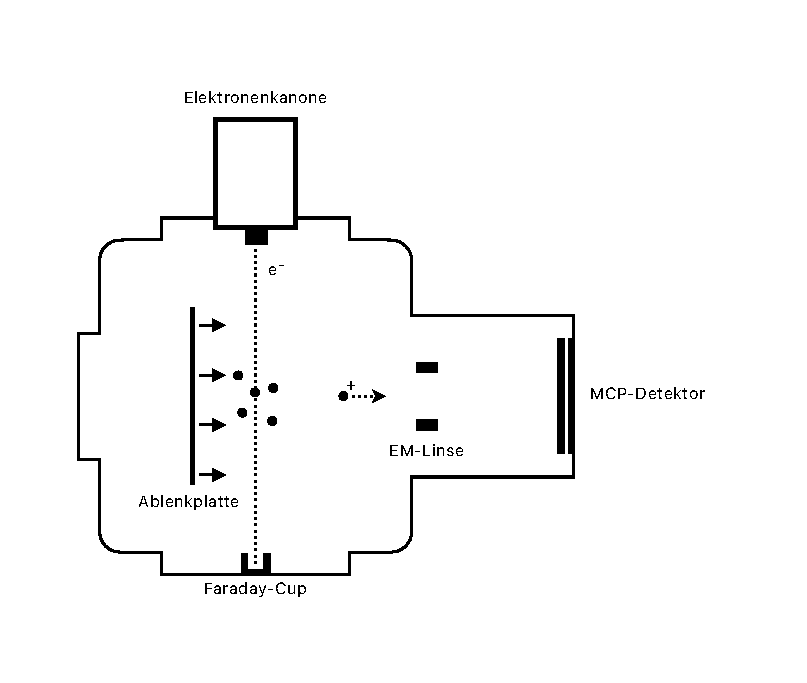
\includegraphics[width=1.2\textwidth]{Zero-B_Aufbau.pdf}
    \caption{Schematischer Aufbau der Zero-B Vakuumkammer und der Elektronenstoßionisation. Die Elektronen werden von der Elektronenkanone erzeugt und auf beschleunigt. Sie stoßen mit den Neutralgasteilchen und ionisieren diese durch Stoßionisation. Die entstehenden Ionen werden durch ein elektrisches Feld auf die Detektorplatten beschleunigt und erzeugen dort ein Signal. Sie können mit einer elektromagnetischen Linse fokussiert werden.}
    \label{fig:Aufbau}
\end{figure}

\section{Detektorsystem}
Bei dem in dieser Arbeit verwendeten Detektor handelt es sich um einen positionssensitiven Mikrokanalplattendetektor (engl. \textit{micro channel plate detector}, MCP-Detektor) der Firma Roentdek. MCP-Detektoren sind eine verbreitete Detektortechnologie, die es ermöglicht den Auftreffzeitpunkt von einzelnen Ionen, Elektronen oder Photonen zu bestimmen. Mit einer Widerstandsanode kann die Position der durch die Platten verstärkten Signale anschließend bestimmt werden. So kann ein \textit{Bild} der detektierten Teilchen erzeugt werden. Ein Goldnetz mit hoher Transparenz (88 \%) schirmt den Detektor von elektromagnetischen Störungen und Restfeldern ab. Der Detektor hat eine aktive Fläche von 80 mm Durchmesser und eine Auflösung von 10 $\mu$m. Die Detektionseffizienz liegt bei in etwa 50 \% und wird von der Transparenz der Detektorplatten bestimmt.

Die Mikrokanalplatten des Detektors dienen der Verstärkung von eintreffenden Singalen über die Erzeugung von Sekundärelektronen. Die Platten bestehen aus Glas, welches mit einer sehr hohen Dichte von kleinen, geraden Kanälen durchzogen ist, welche die gegenüberliegenden Seiten verbinden. Bei der Herstellung wird das Glas dafür, ähnlich wie bei der Herstellung von Glasfasern, gezogen und in bis zu 1 mm Dicke Scheiben geschnitten. Der Durchmesser der Kanäle liegt bei einigen Mikrometern. Die Innenwände der Kanäle bestehen aus einem halbleitendem Material, an welches eine Spannung entlang der Kanäle angelegt wird. Diese beschleunigt die Elektronen entlang des Kanals. Trifft ein Teilchen auf die Wand eines Kanals der Detektorplatten, löst es Sekundärelektronen durch Stoßionisation aus. Diese stoßen entlang des Kanals wiederum mit der Wand und es entsteht eine Elektronenlawine. Diesen verstärkenden Effekt macht man sich zunutze, um aus einzelnen Teilchen eine messbare Ladungswolke zu erzeugen. Um die Wahrscheinlichkeit einer Kollision einfallender Teilchen mit den Kanalwänden zu steigern, sind die Kanäle um etwa \ang{10} gegenüber der Flächennormalen geneigt. 

Typischerweise werden zwei MCPs hintereinander verwendet, wobei sie um \ang{180} zueinander gedreht sind. Sie befinden sich in einer sogenannten \textit{Chevron}-Konfiguration. Die zweite Platte wird verwendet, um die Verstärkung weiter zu erhöhen und Ionen-Feedback zu minimieren. Ionen-Feedback beschreibt das Zurückfließen von Ionen in die Kammer. Die hohe Anzahl an Elektronen in den Kanälen der MCPs können Restgas ionisieren, welches dann aufgrund der Beschleunigungsspannung rückwärts durch die Kanäle in die Kammer gelangen könnte. 

Wie in \cite{Detektorsystem} dargestellt, gibt es unterschiedliche Ansätze die zweidimensionale Positionsinformation der durch die Platten erzeugten Ladungswolke zu ermitteln. Der für das Experiment verwendete Detektor ist ein \textit{delay-line} Detektor, genauer der \textit{DLD80} von Roentdek. Das Konzept macht sich zu Nutzen, dass eine auf ein Drahtgitter treffende Ladungswolke ein elektrisches Signal in den Leitern erzeugen. Dieses hat eine Laufzeit in der Größenordnung einier Nanosekunde bis es an den Enden des Leiters ankommt. Anhand dieser Laufzeitdifferenz kann die Position auf dem Detektor in einer Dimension bestimmt werden. Mithilfe eines zweiten, um \ang{90} gedrehten, Leiters, kann die Position zweidimensional dargestellt werden. Der Detektor hat eine aktive Fläche mit einem Durchmesser von 80 mm.

\begin{figure}
    \centering
    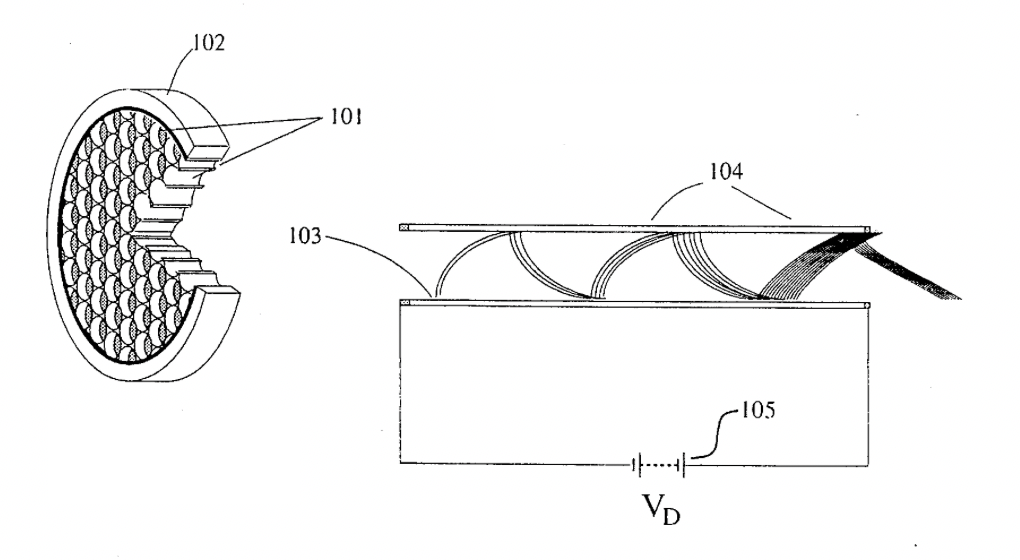
\includegraphics[width=.8\textwidth]{MCP.png}
    \caption{Schnitt und Funktionsprinzip einer MCP aus \cite{MCP}, hier dargestellt mit einem eintretenden Elektron. (102) Haltungsflange, (101) Mikrokanäle aus Glas, (103) Elektron, welches in den Kanal eintritt, (104) erzeugte Sekundärelektronen, (105) Spannungsversorgung der Platten}
    \label{fig:MCP} 
\end{figure}

\begin{figure}
    \centering
    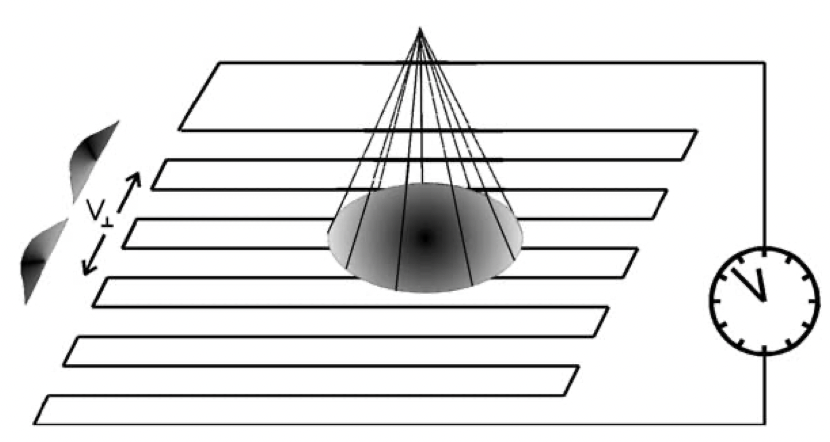
\includegraphics[width=.6\textwidth]{DLD.png}
    \caption{Funktionsprinzip der Laufzeitmessung in einer Dimension aus \cite{Detektorsystem}. Der Leiter ist mäanderförmig aufgebaut, um die Laufzeit zu verlängern und die Positionsgenauigkeit zu erhöhen. Das Signal propagiert in beide Richtungen mit der effektiven Geschwindigkeit $v_\perp$.}
    \label{fig:DLD} 
\end{figure}

\section{Konditionierung des Detektors}
Nachdem der Detektor eingebaut ist, muss er einer Konditionierung unterzogen werden, damit er ohne Risiko beschädigt zu werden verwendet werden kann. Zur Konditionierung soll die Spannung zwischen den MCPs in 100 V Schritten erhöht werden und je für einige Minuten konstant gelassen werden. Das hat den Hintergrund, dass Partikel, wie zum Beispiel Staubteilchen, sich von den MCPs oder Teilen des Detektors lösen können und bei schnellem Ansteigen der Spannung Schaden an den Platten hinterlassen können. Beim Konditionieren können diese Partikel sich nach und nach lösen und bekommen nur minimale kinetische Energie zugeführt. Außerdem können Überschläge bei möglichst geringer Potenzialdifferenz festgestellt werden, welche ebenfalls von Partikeln begünstigt werden können. Für die Spannungsversorgung der Detektorplatten wird eine Hochspannungsquelle verwendet, die mit einem Überstromschutz bei sprunghaft ansteigendem Strom abschaltet. Bei einem Vakuum mit einem Druck kleiner als 10$^{-6}$ mBar kann die Konditionierung begonnen werden und wird über mehrere Stunden durchgeführt bis zu einer Potenzialdifferenz von 2,7 kV. Nach jedem Erhöhen der Spannung wird der sich eingestellte Strom notiert. Mit Strom und Spannung kann über das Ohm'sche Gesetz der Widerstand berechnet werden, welcher in etwa konstant bleiben oder sich mit steigender Spannung etwas verkleinern sollte. Tabelle \ref{tab:Konditionierung} im Anhang zeigt die notierten Werte für die Konditionierung ab 880 V, welche ohne Probleme durchgeführt werden konnte. Nach einmaliger Konditionierung kann der Detektor mit einer Geschwindigkeit von etwa 40 V/s ohne weiteres hochgefahren werden.

\section{Signalverarbeitung}
Die auf der Anode des Detektors entstehenden Signale müssen weiterverarbeitet werden, um sie für die Auswertung zu nutzen. Ein Großteil der Signalverarbeitung wird in dieser Arbeit analog umgesetzt. Viele der verwendeten Geräte sind ältere, aber verlässliche Nuclear Instrumentation Module (NIM). Diese können sehr modular in einem Rack verbaut und über BNC-Kabel verbunden werden. Im Folgenden wird die Signalverarbeitung zur Flugzeitmessung und die zur positionssensitiven Auflösung der Ionen unterschieden.

\subsection{Flugzeitmessung}
Eine schematische Übersicht der Verarbeitung ist in Abbildung \ref{fig:ToF} zu finden. Der Signalfluß, angefangen mit dem Detektor wird nun beschrieben.


\begin{figure}
    \centering
    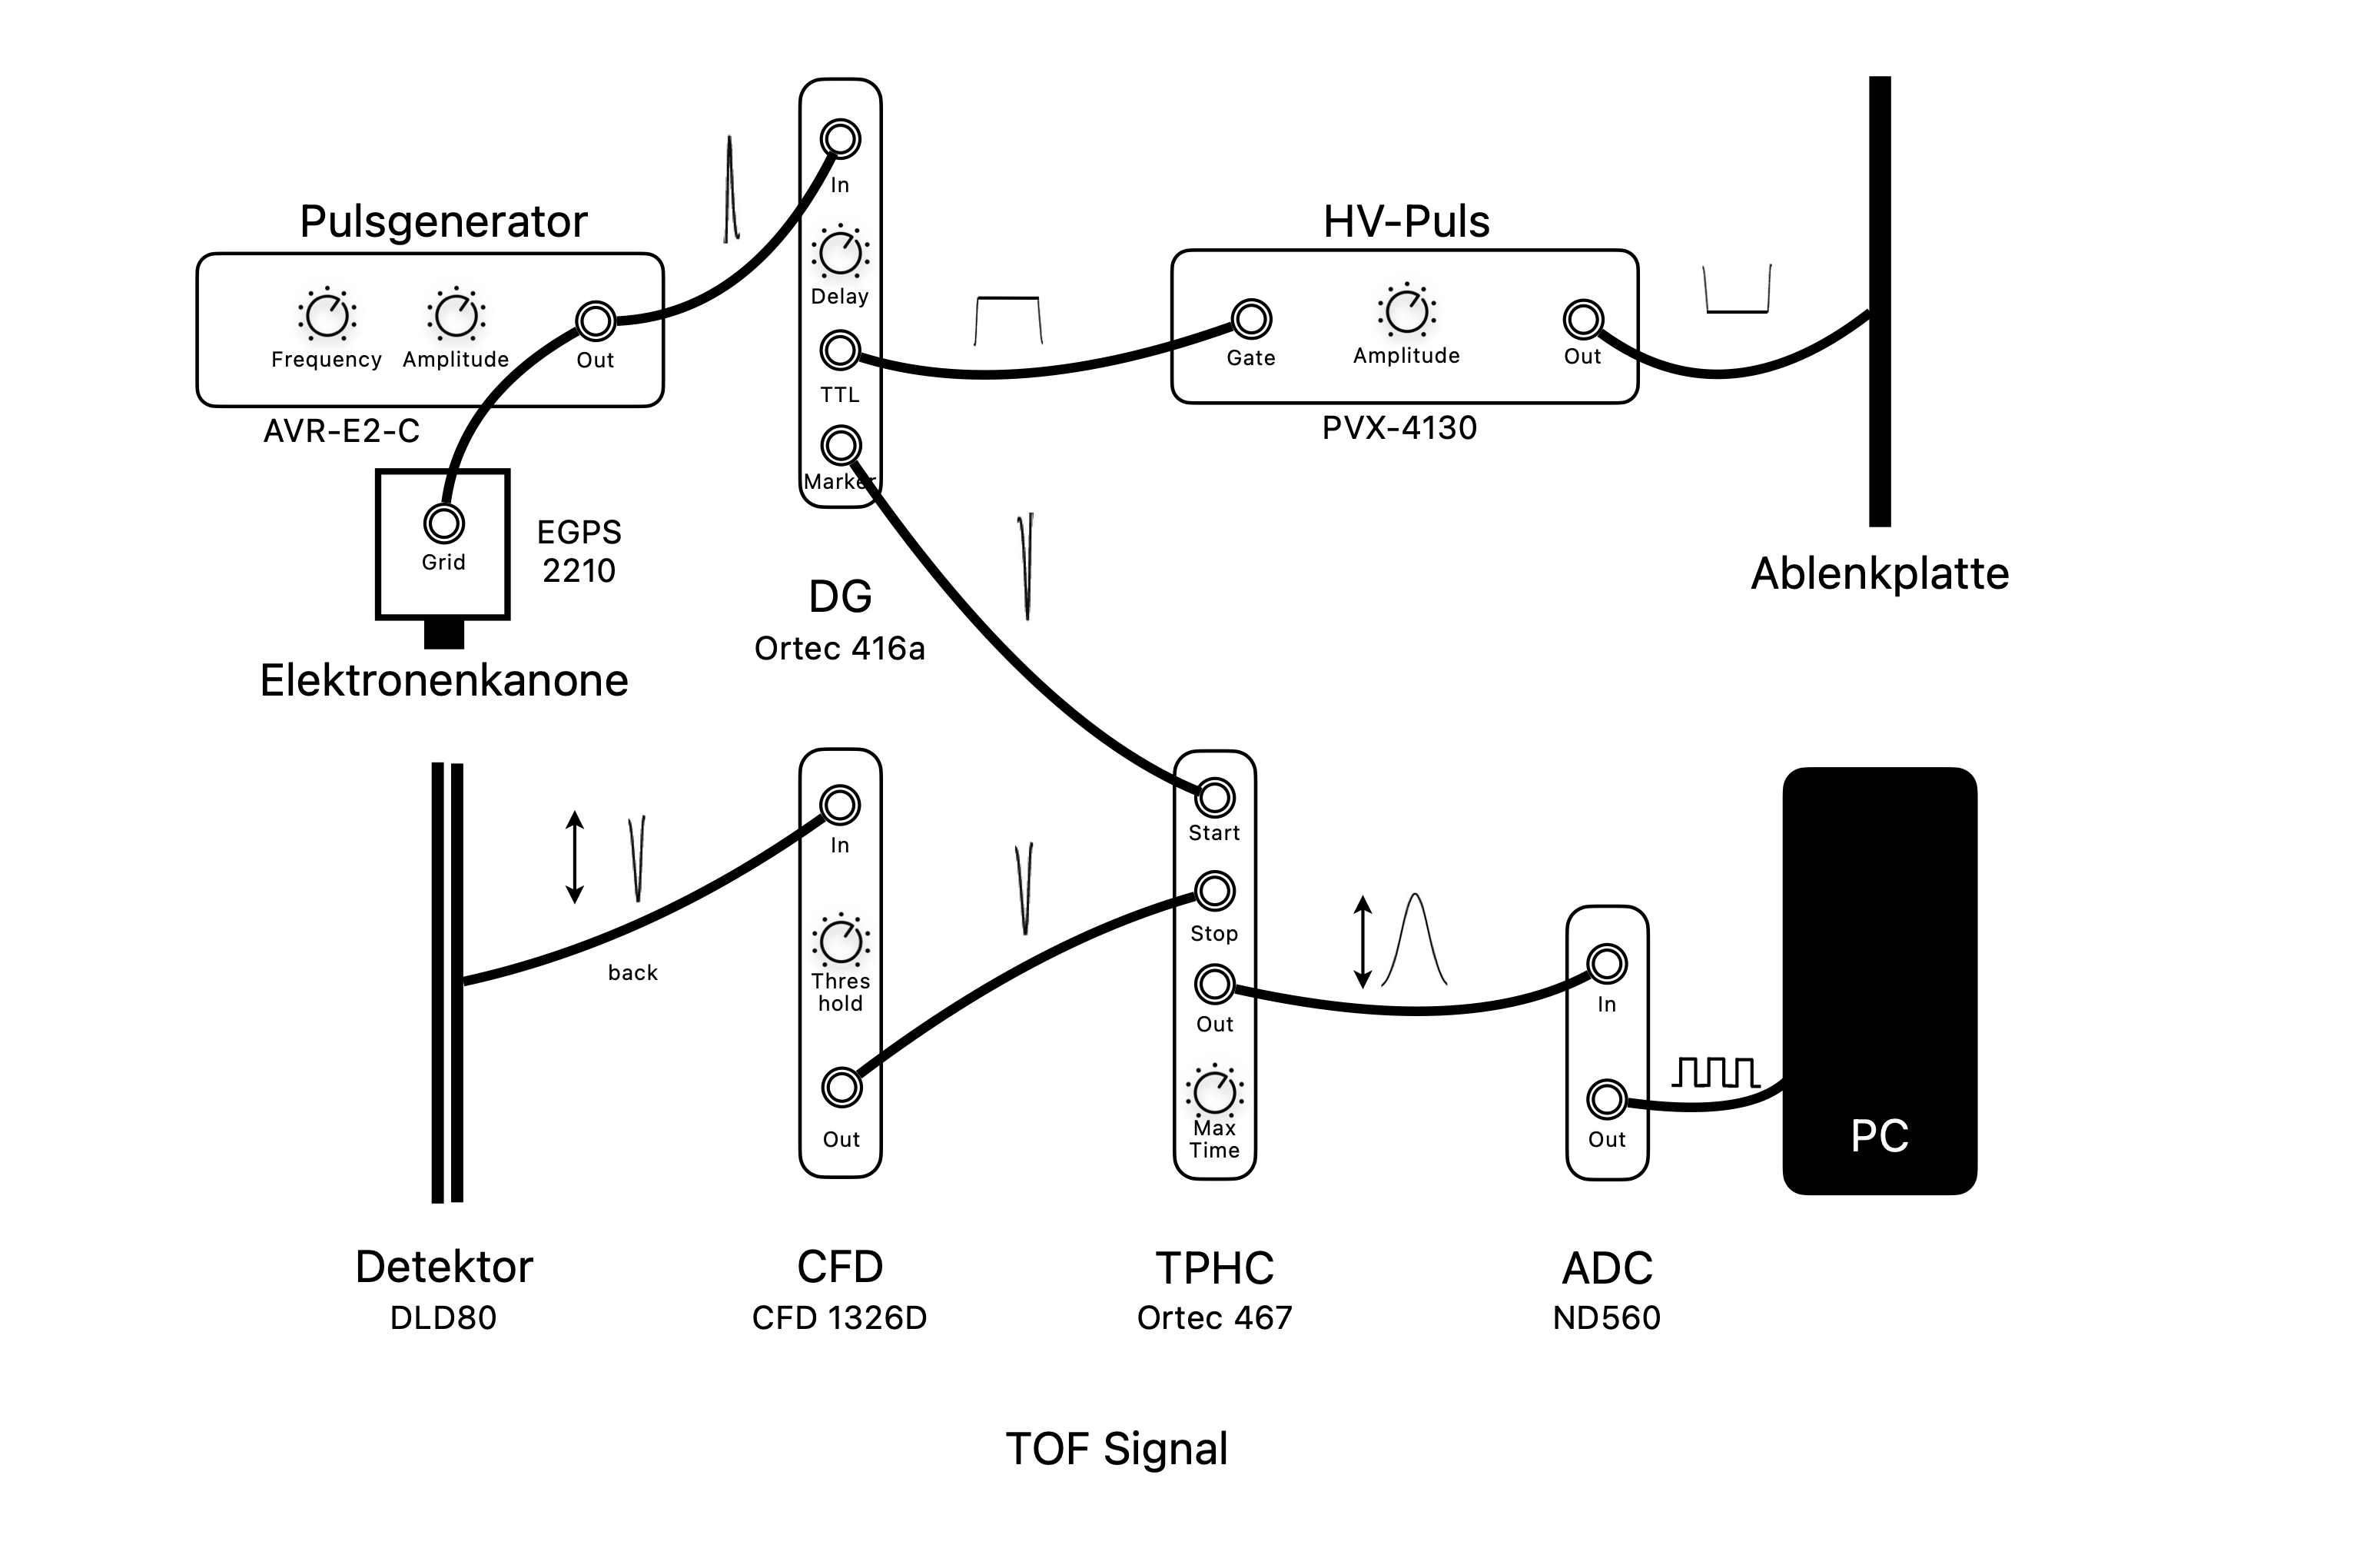
\includegraphics[width=1\textwidth]{ToF_Signals.png}
    \caption{Schematisch dargestellter Signalfluß der ToF-Messung. Der Signalfluß erfolgt, mit Ausname der Elektronenkanone, von links nach rechts. Die verwendeten Geräte sind stark vereinfacht abgebildet, wobei die wichtigsten Einstellungen inkludiert wurden. Die jeweilige Form der Signale ist über den Verbindungen gezeigt und ist rein qualitativ. Power Supplies sowie Anzeigegeräte sind nicht abgebildet.}
    \label{fig:ToF} 
\end{figure}

Für die Flugzeitmessung wird vom Detektor ein Spannungssignal ausgegeben, das von einem Ion beim Auftreffen auf die Anode erzeugt wird.  Der Pegel hängt von der kinetischen Energie des Ions ab und hat eine gewisse Varianz. Der Zeitpunkt soll möglichst unabhängig vom Pegel bestimmt werden können. Legt man also lediglich einen Schwellwert (engl. \textit{Threshold}) fest, variert der Zeitpunkt mit der Steilheit der Flanke. Um den Zeitpunkt unabhängig vom Pegel zu bestimmen, wird ein Constant Fraction Discriminator (CFD) verwendet. Dieser erzeugt ein Ausgangssignal, sobald ein bestimmter Bruchteil des Signals erreicht wird. Abbildung \ref{fig:CFD} zeigt das Prinzip des CFD. Dafür wird im CFD das einlaufende Signal verzögert und mit dem Originalsignal über einen Differenzverstärker verrechnet. So ergibt sich ein Nulldurchlauf der Spannung, der von der Verzögerung abhängt, nicht aber von der Amplitude. 

Der über den CFD ermittelte Auftreffzeitpunkt kann dann als Stoppsignal für die Flugzeitmessung dienen. Um die Information über die Zeitdifferenz zwischen dem Start- und Stoppsignal zu erhalten, wird ein Time-to-Pulse-Height (TPHC) Modul verwendet. Dieses erzeugt ein Signal, dessen Höhe proportional zur Differenz eines Start und Stopp Pulses ist. Der 

\begin{figure}
    \centering
    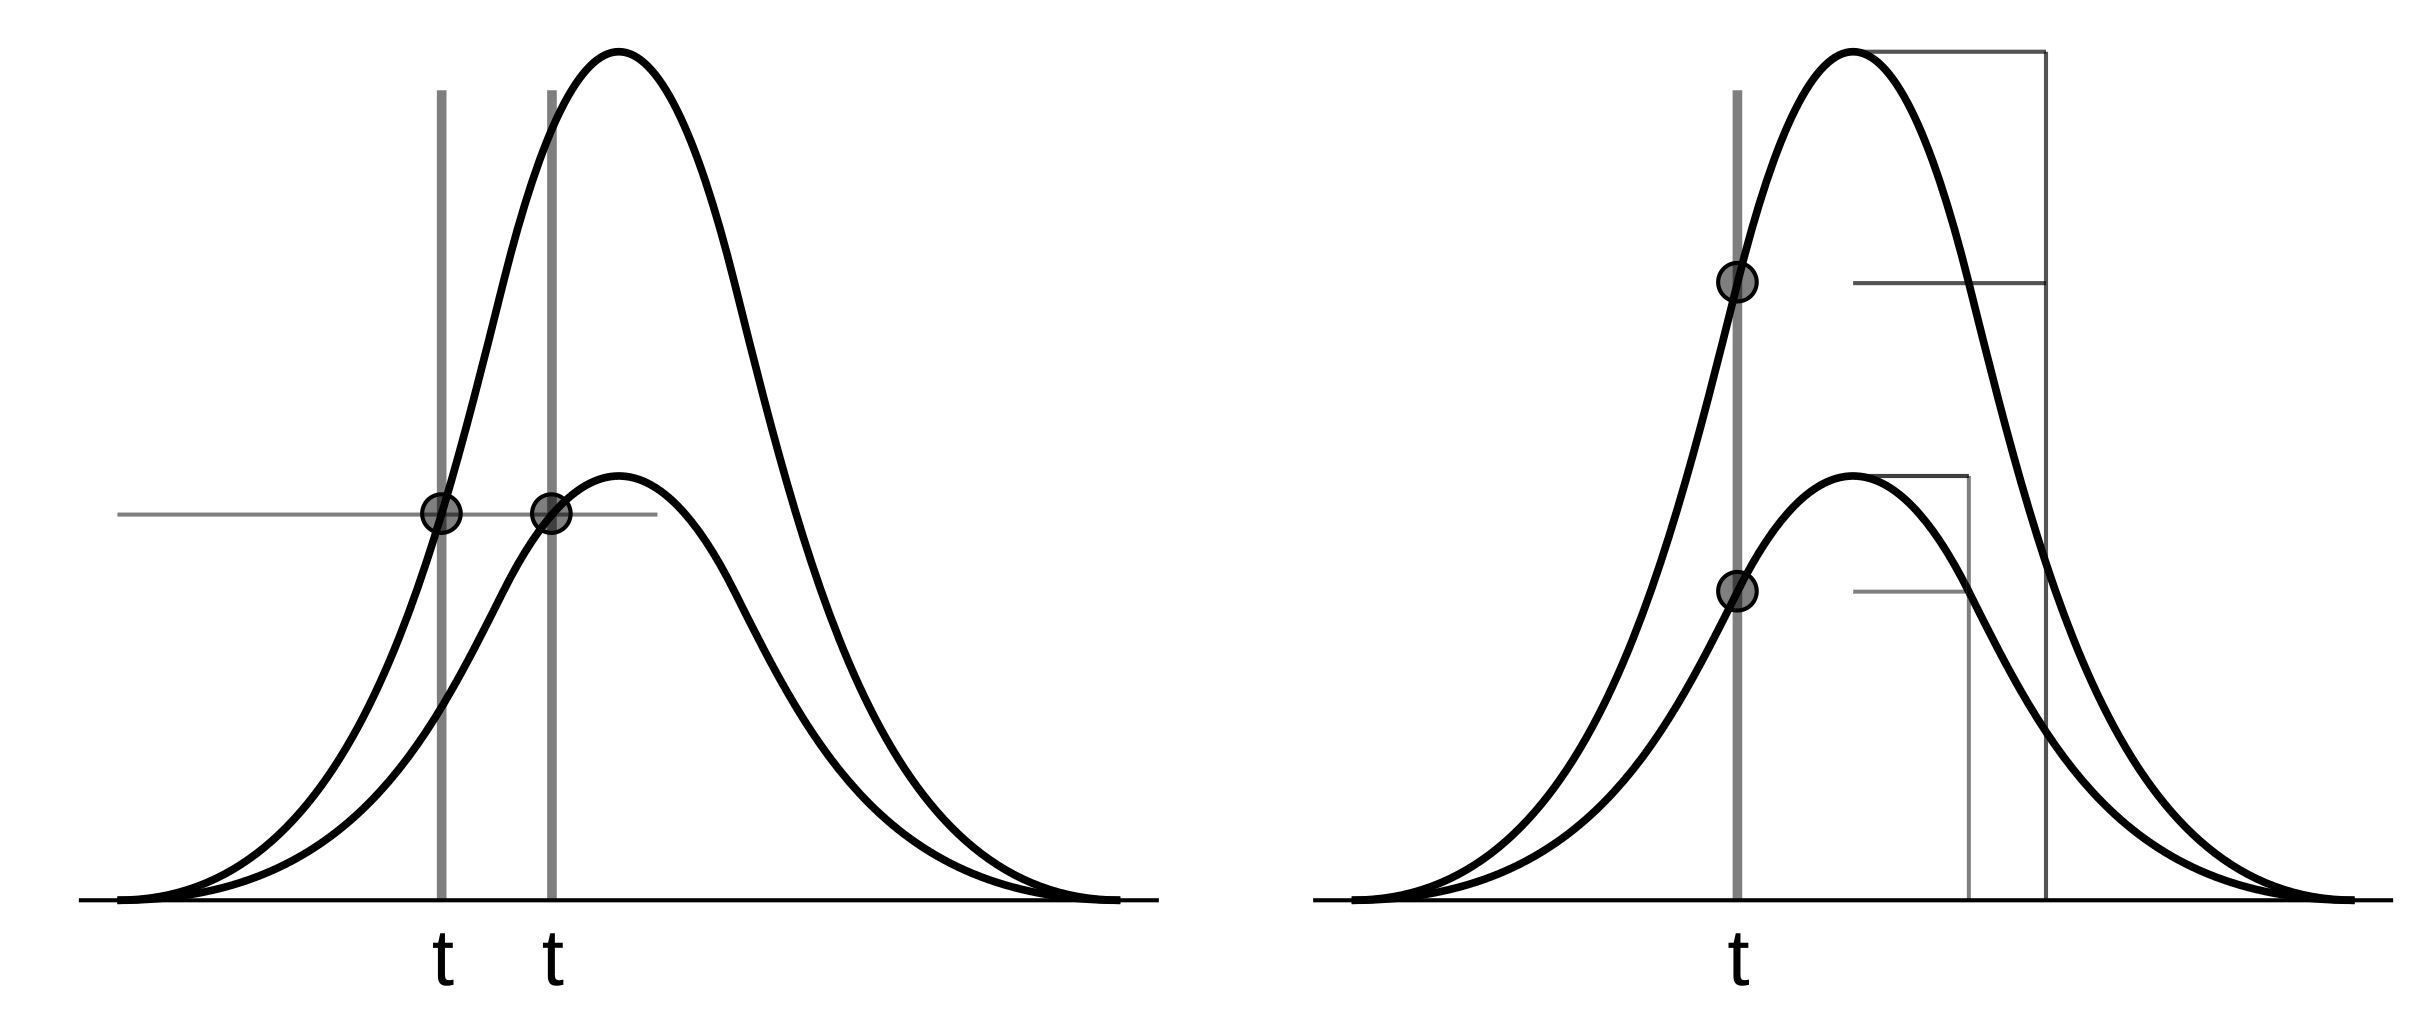
\includegraphics[width=.8\textwidth]{cfd.png}
    \caption{Prinzip des Constant Fraction Discriminators. Links: Zeitpunkte beim Überschreiten eines Schwellwertes sind unterschiedlich, rechts: der Zeitpunkt beim Überschreiten eines Bruchteils des Signals ist unabhängig vom Pegel.\\
    \small Quelle: https://commons.wikimedia.org/w/index.php?curid=534201}
    \label{fig:CFD} 
\end{figure}


\begin{figure}
    \centering
    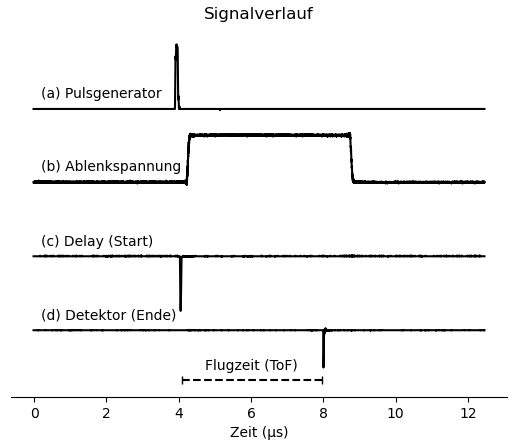
\includegraphics[width=1\textwidth]{Signalverlauf.png}
    \caption{aufgenommenener Verlauf der relevanten Signale. (a) zeigt den initialen Spannungspuls aus dem Pulsgenerator, mit dem auch die Elektronenkanone getriggert wird. Über einen Delay-Generator wird das verspätete Signal (c) erzeugt, um die Ablenkspannung (b) anzusteuern. (d) zeigt das Signal, welches auf der Anode des Detektors entsteht, nachdem es durch den CFD gelaufen ist. Die zeitliche Differenz aus (c) und (d) entspricht der Flugzeit}
    \label{fig:Signal} 
\end{figure}

\subsection{Positionssensitive Auflösung}
Sie werden bereits in der Elektronik des Detektors verstärkt, wobei darauf geachtet werden muss, dass die Pulse nicht den Verstärker sättigen. Ihre Höhe hängt von der Spannung auf der Front-Platte des Detektors ab und RoentDek empfielt die Differenz nicht höher als 2600 V zu wählen. 